\newpage\phantomsection

\begin{appendices}

\makeatletter
	\def\toclevel@chapter{1}
\makeatother

% \makeatletter
% 	% \addappheadtotoc
% 	\addtocontents{toc}{\let\protect\l@chapter\protect\l@section}
% 	% \xpatchcmd{<cmd>}{<search>}{<replace>}{<success>}{<failure>}
% 	\xpatchcmd{\Hy@org@chapter}{{toc}{chapter}}{{toc}{section}}{}{}%
% 	\xpatchcmd{\Hy@org@chapter}{{toc}{chapter}}{{toc}{section}}{}{}%
% \makeatother

%% ================================================================== Appendix A

% \chapter{Published Papers}
% \label{appendix:publications} % Linked in LOP
% 
% Copies of published papers are provided here for reference. These
% papers cover the following topics:
% 
% \begin{itemize}
%     \item Development of HEATHER
%     \item Development and validation of the guinea pig model (latest submitted
%     revision)
%     \item Incorporating vascular structures in the proof of concept (POC) model
%     \item Influence of blood vessels in HEATHER
%     \item Time-domain model of electrochemistry at the electrodes
%     \item Frequency-dependent simulation in the POC model
%     \item Effects of electrode recessing on safety
% \end{itemize}
% 
% 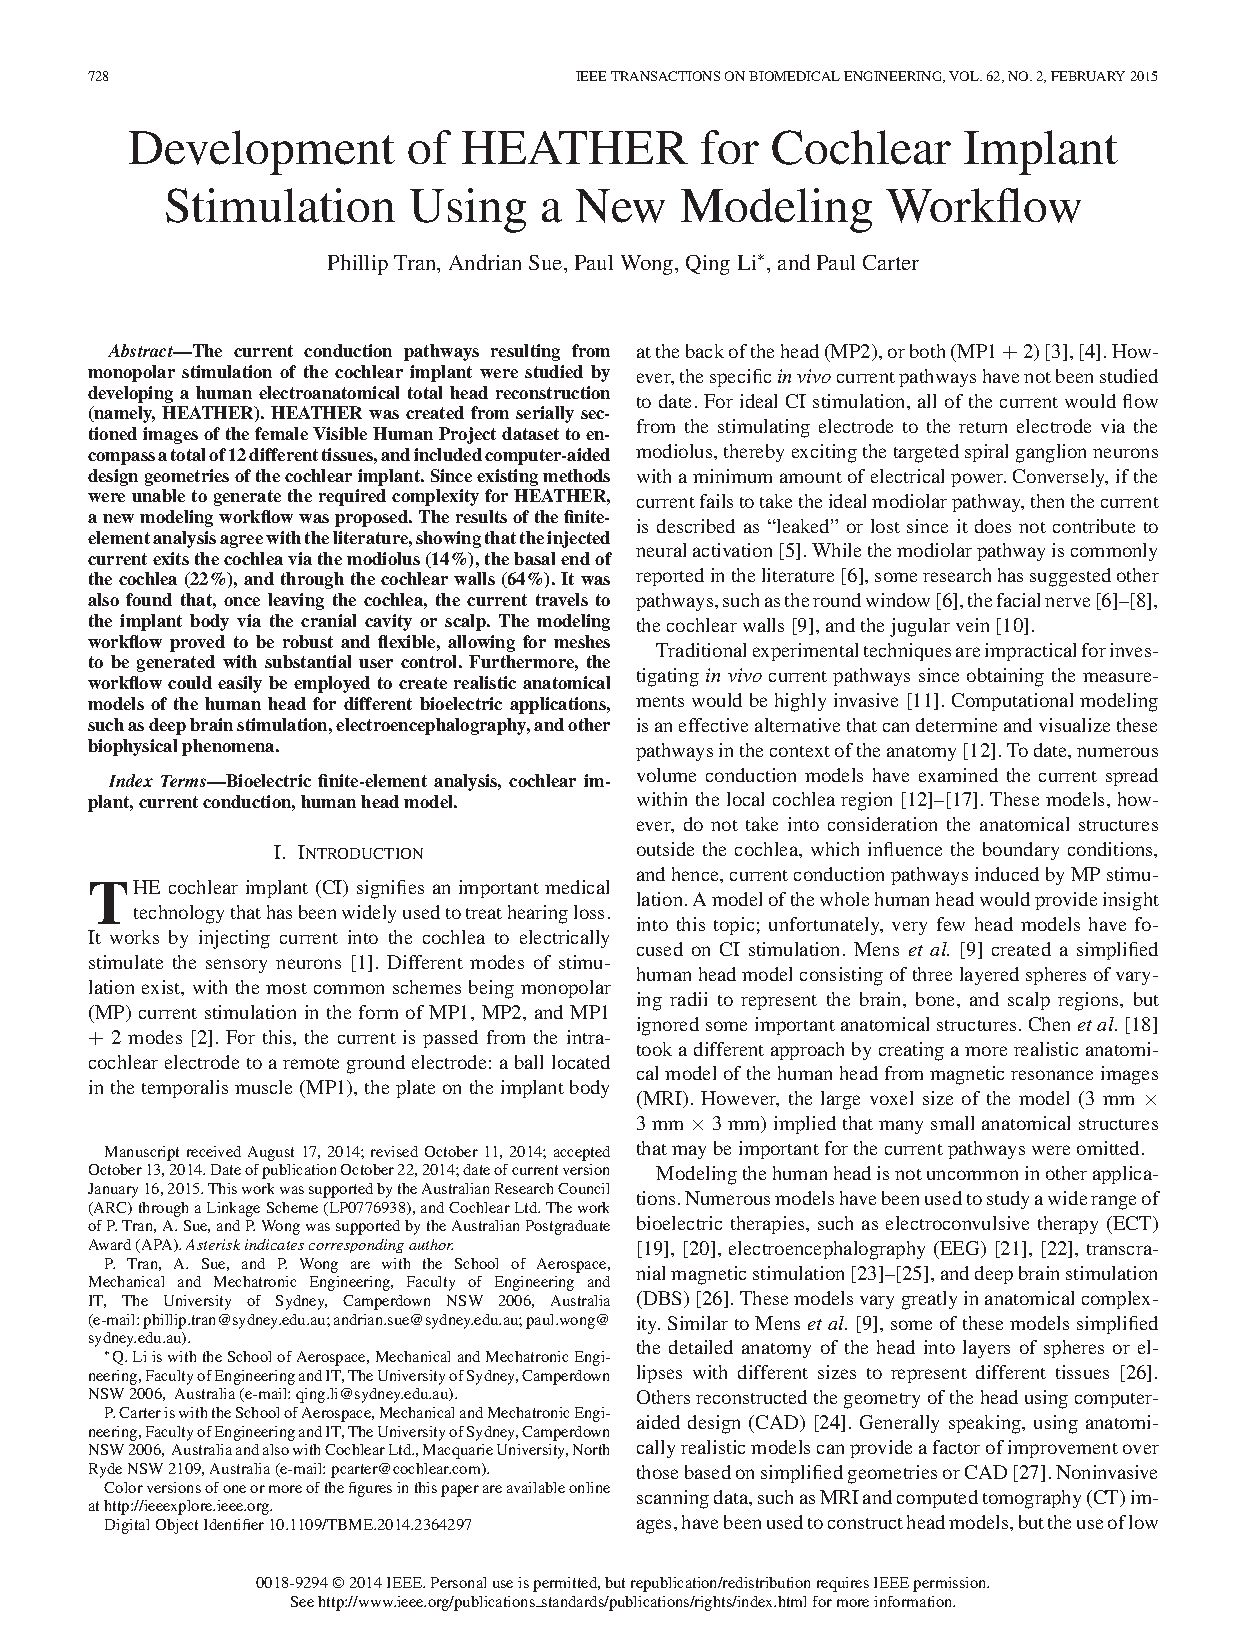
\includepdf[pages=-]{Appendix/Tran_2015_HEATHER.pdf}
% 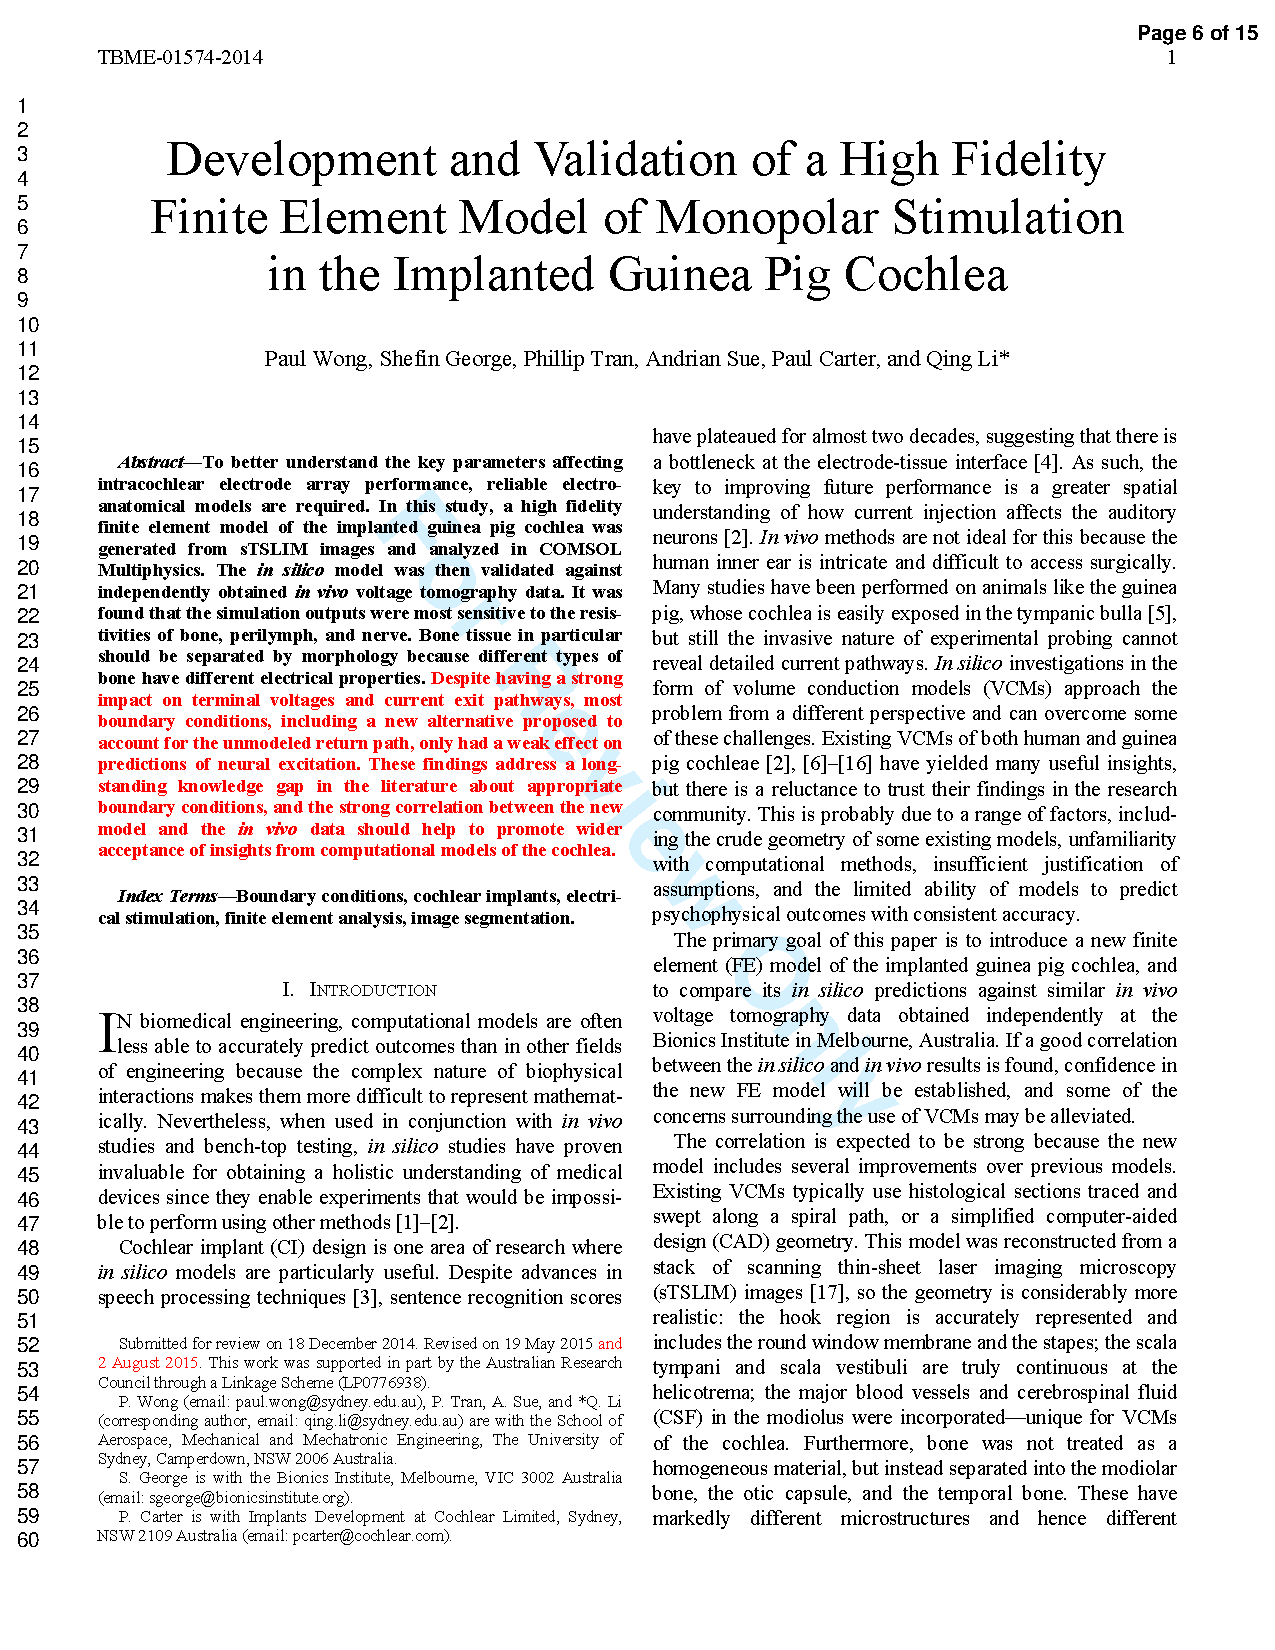
\includepdf[pages=-]{Appendix/Wong_2015_Development.pdf}
% 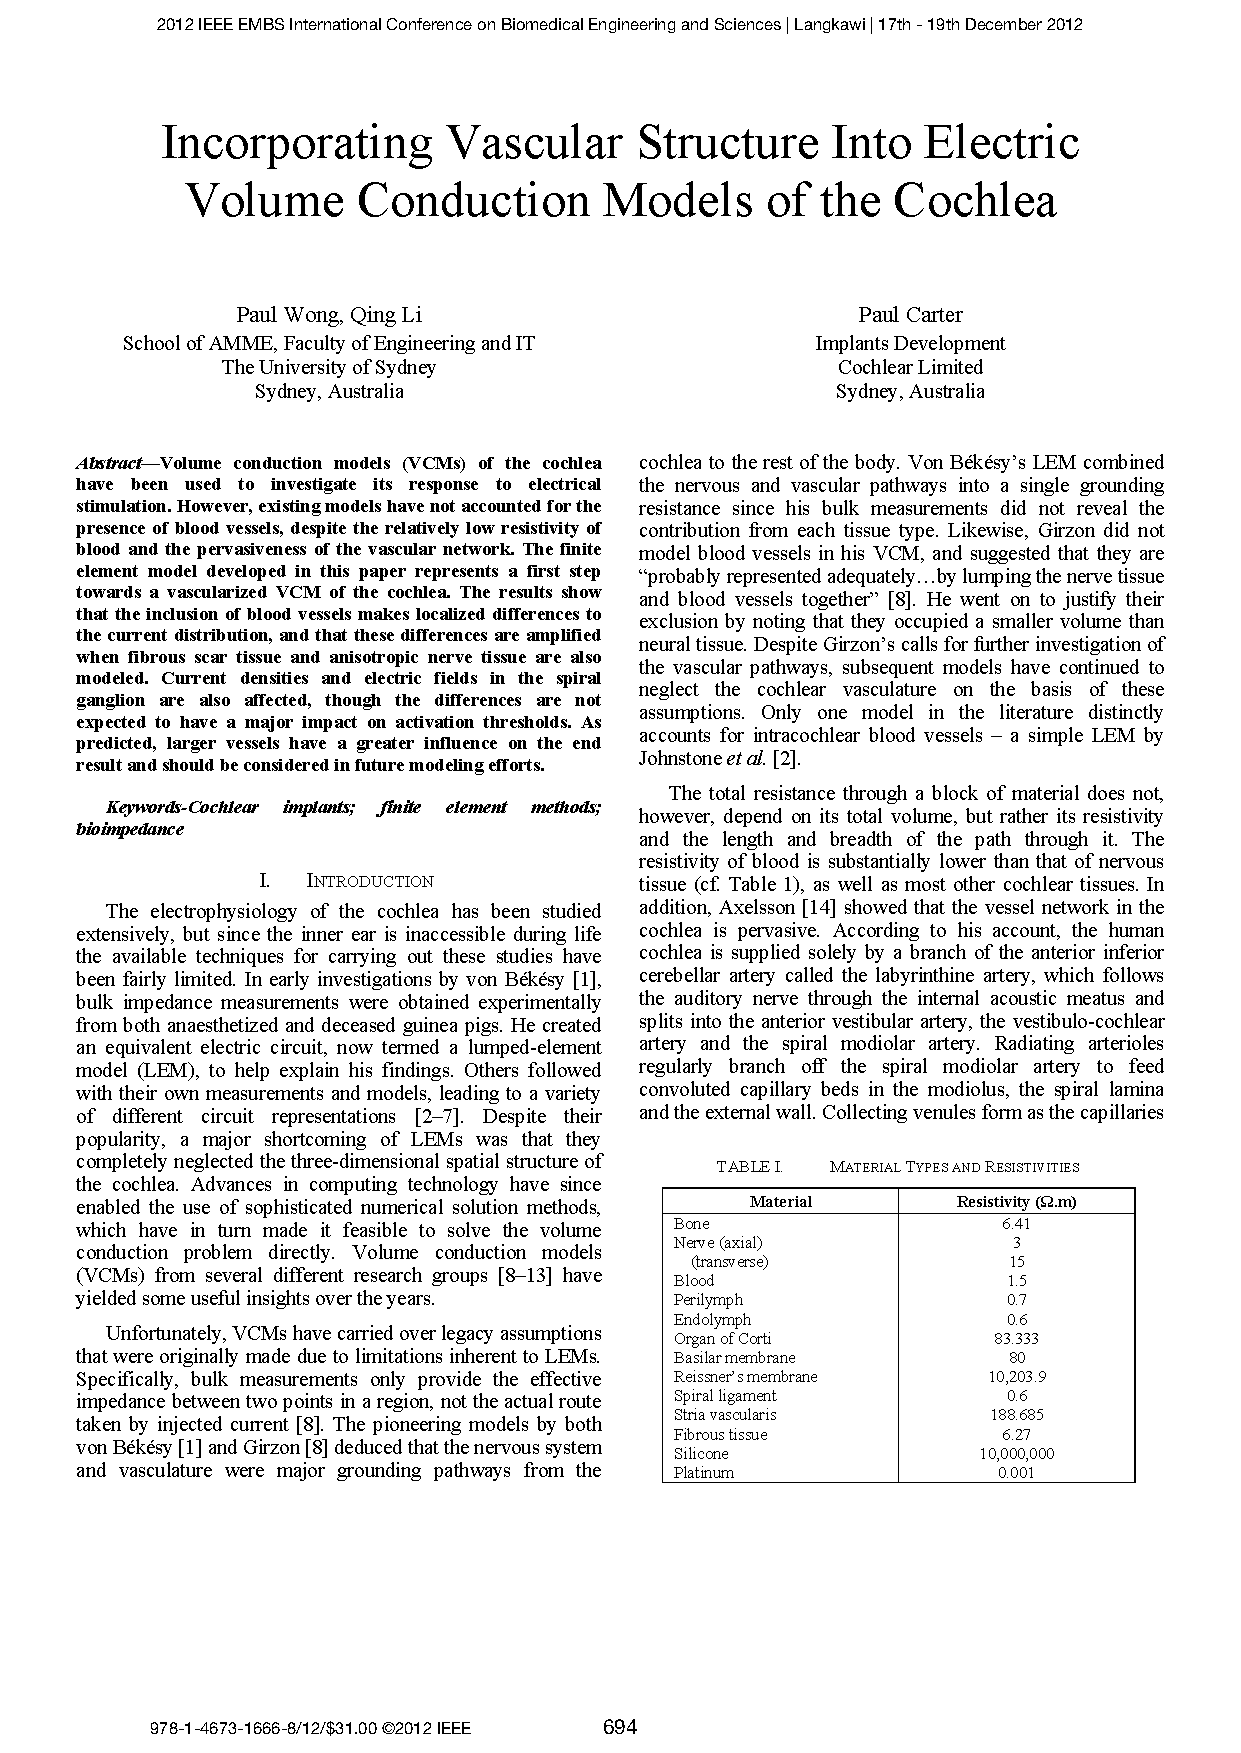
\includepdf[pages=-]{Appendix/Wong_2012_IECBES2012.pdf}
% 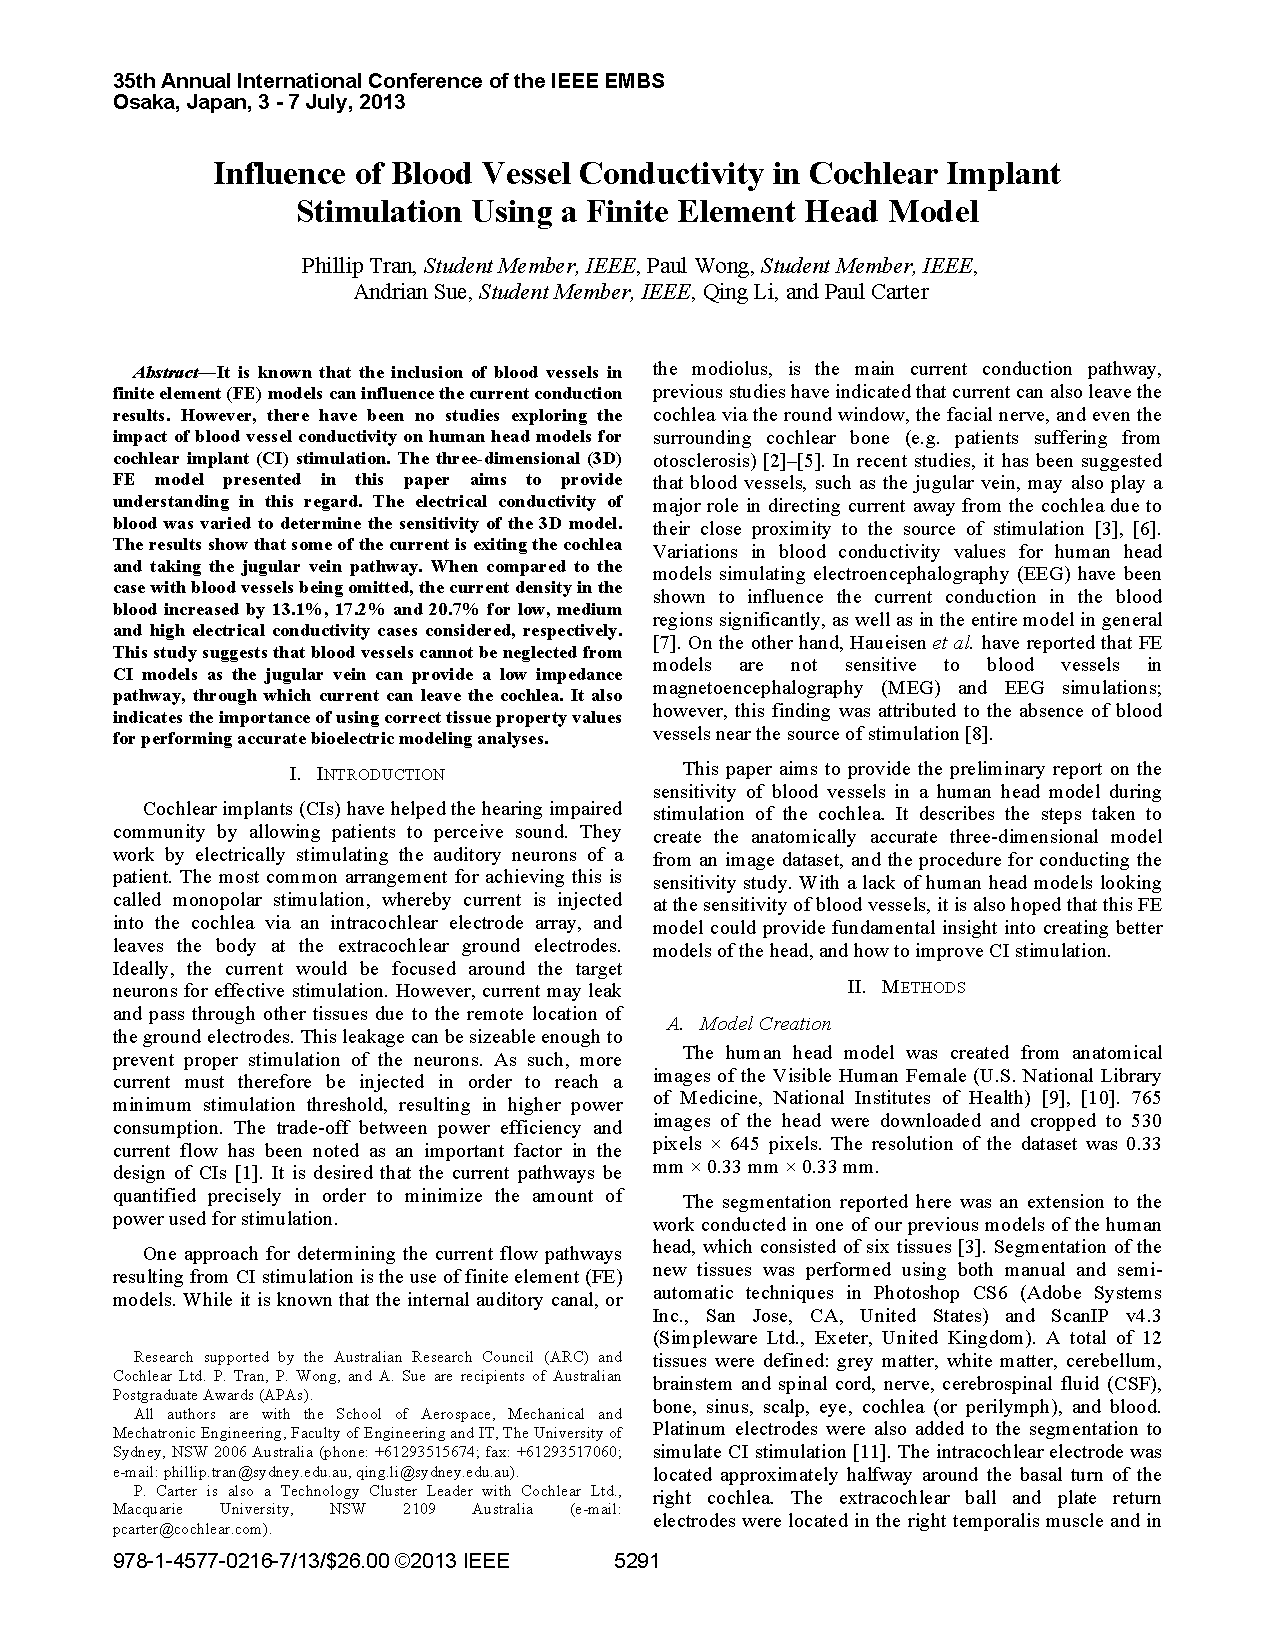
\includepdf[pages=-]{Appendix/Tran_2013_BloodVessel.pdf}
% 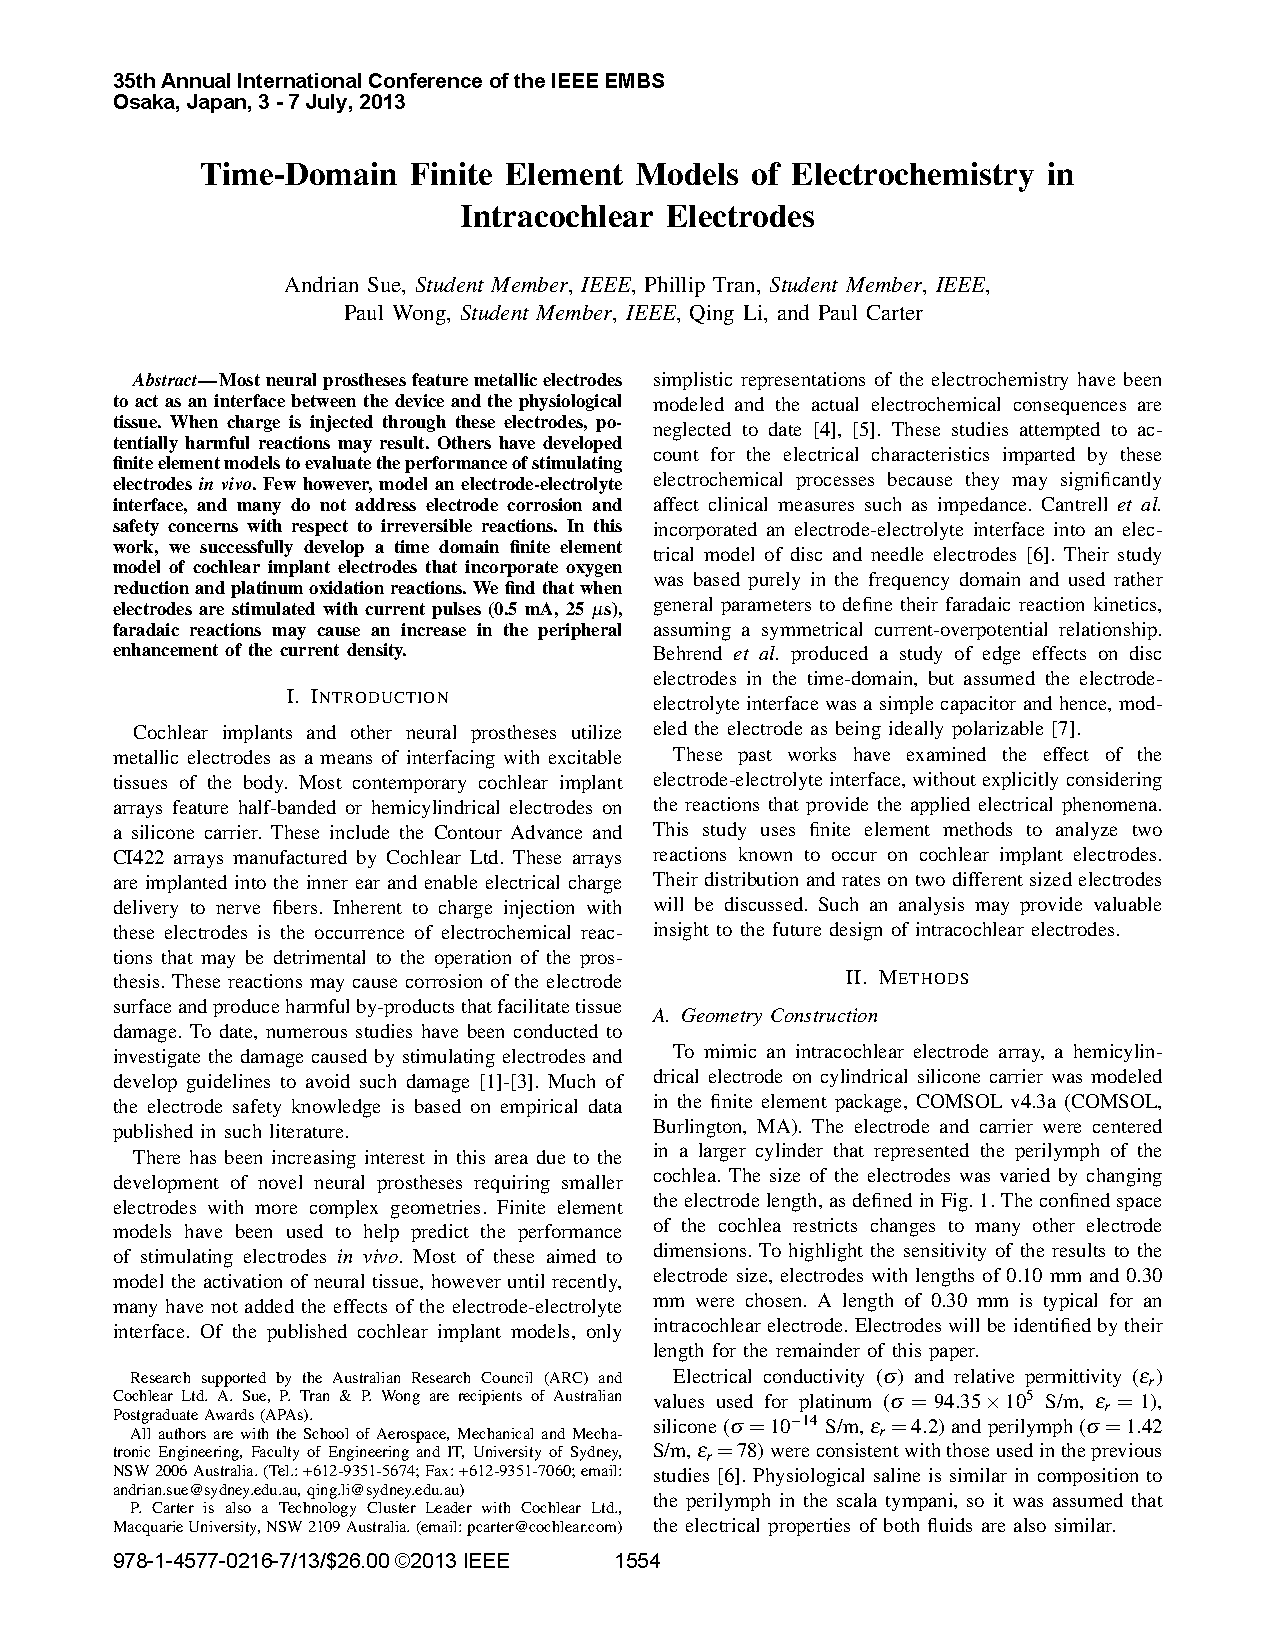
\includepdf[pages=-]{Appendix/Sue_2013_TimeDomain.pdf}
% 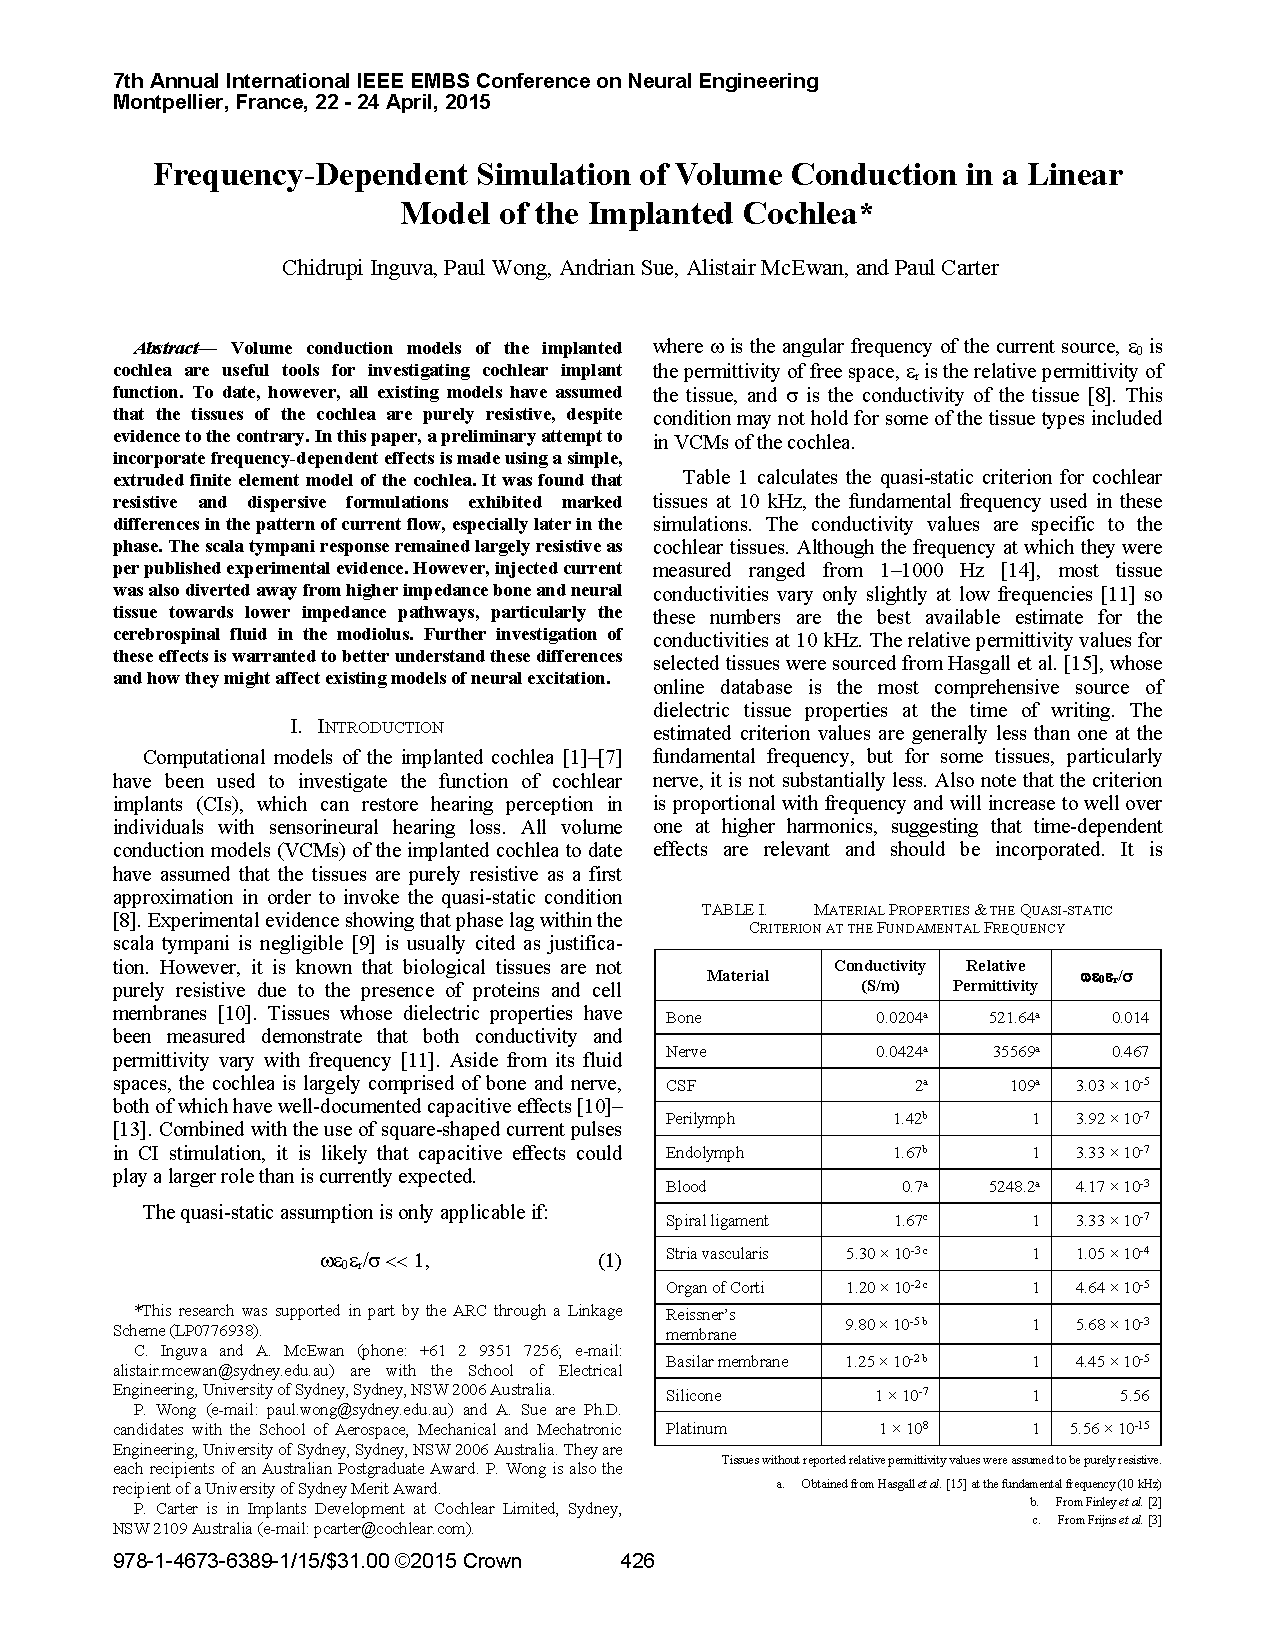
\includepdf[pages=-]{Appendix/Inguva_2015_Frequency.pdf}
% 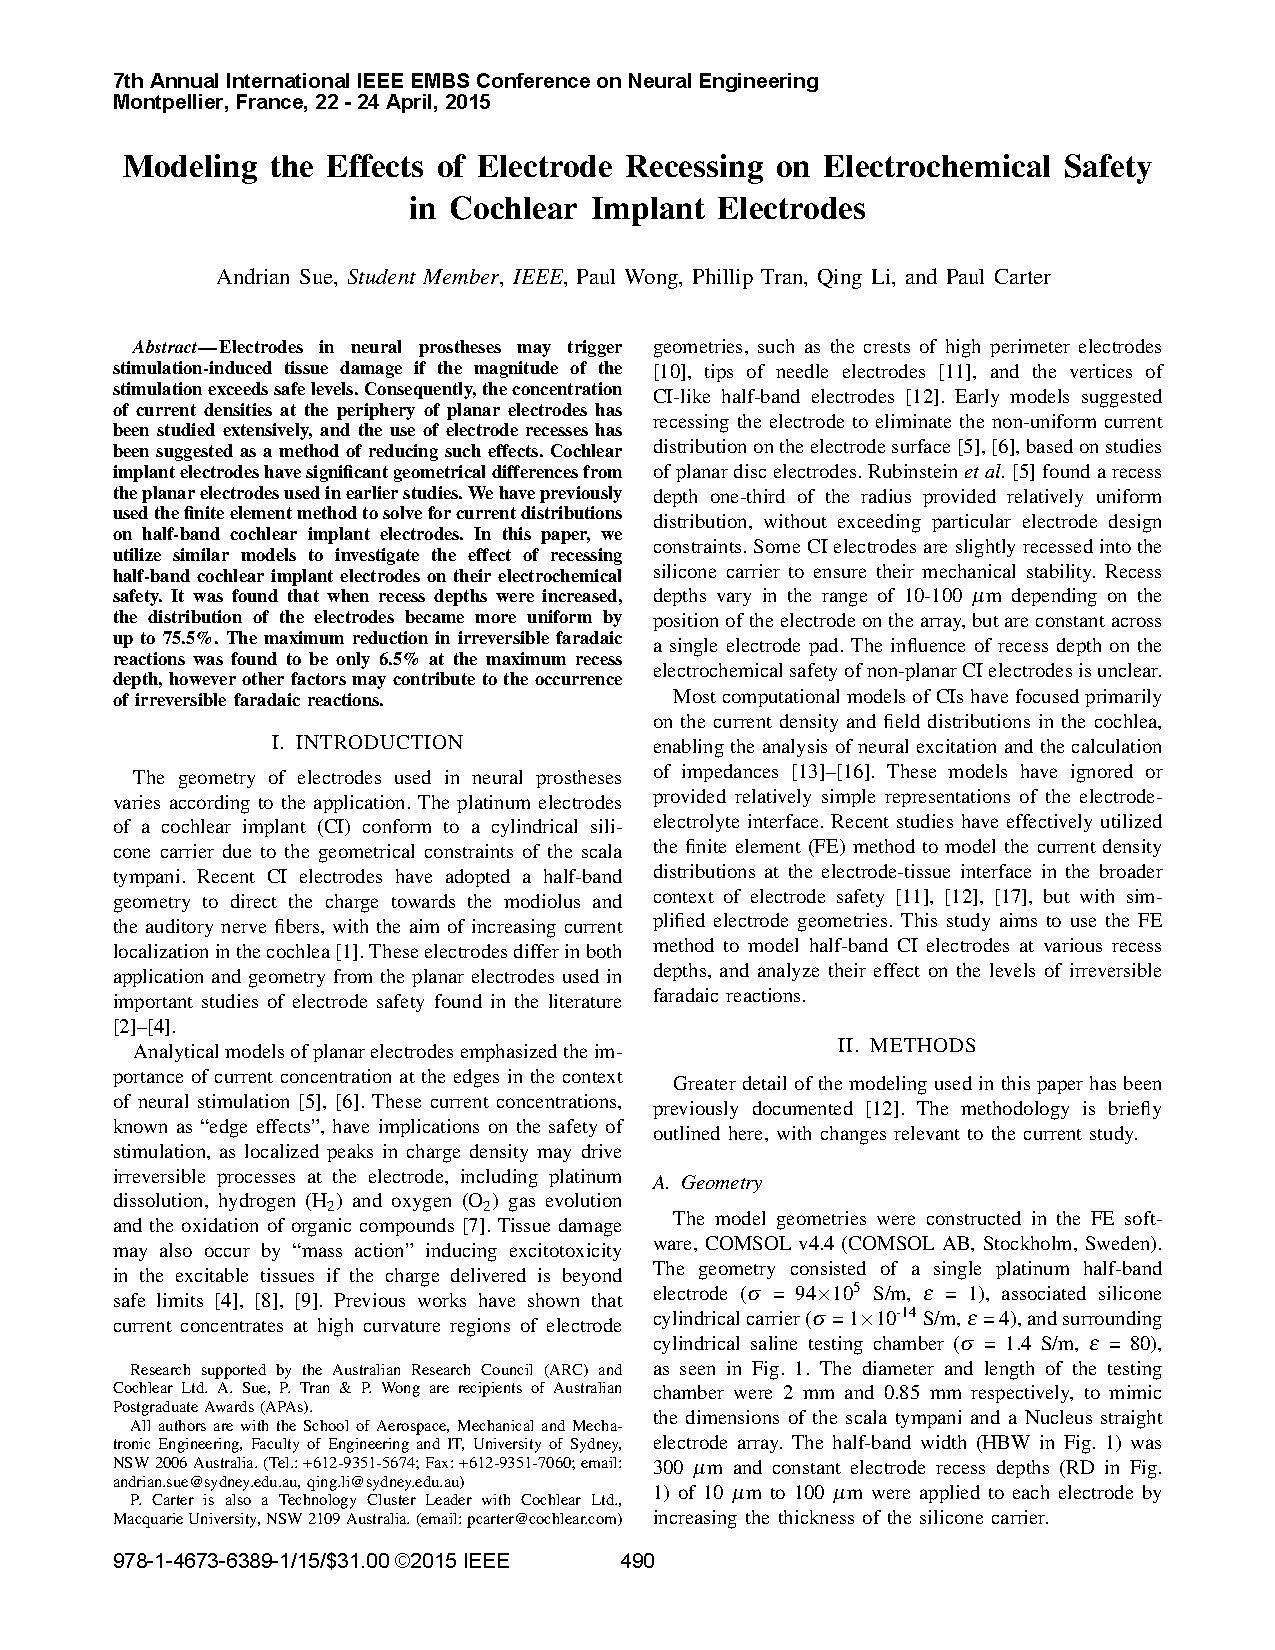
\includepdf[pages=-]{Appendix/Sue_2015_Recessing.pdf}

%% ================================================================== Appendix B

\chapter{MATLAB Function Licences}
\label{appendix:licences} % Linked in Model Dev

% Separate formatting
\setstretchcode

interparc.m
\lstinputlisting[]{Code/interparc_license.txt}

\clearpage

arclength.m
\lstinputlisting[]{Code/arclength_license.txt}

\setstretchnormal

%% ================================================================== Appendix B

\chapter{Streamline Seeding}
\label{appendix:streamline_seeding} % Linked in Validation

% \section{The Problem with Seeding on Selected Boundaries}

For this thesis, we wanted to know what path injected current follows after it
leaves the stimulating electrode. This was in fact one of the earliest questions
von \bekesy{} raised in his research~\cite{vonbekesy1951}. While the technology
of his time was limiting, there are now a variety of tools that are able to
visualise current pathways in an intuitive and meaningful manner.

One of the main reasons COMSOL was chosen was because it offers an easy way to
generate such streamline plots. These plots trace the path of the vector field
through the volume, based on a set of seed points. The streamlines should
obviously be seeded on the exposed surface of the active electrode. COMSOL
provided several options for streamline seeding. At first, we chose to start the
streamlines ``on selected boundaries'' because that option allowed the number of
streamlines desired to be set. However, it soon became apparent that there were
some problems with this approach because it did not clearly define how the seed
points were distributed spatially over the selected surface.

From our observations, it appeared that the the seeding algorithm was based on
the mesh nodes on the selected surface. (Keep in mind that a pre-meshed volume
was imported, so COMSOL was unaware of the underlying geometry.) The problems
were therefore twofold (see
Figure~\ref{fig:seeding_problem_rand1}--\ref{fig:seeding_problem_rand3}).
Since the Octree algorithm used tetrahedral elements, the nodes on the electrode
surfaces were not aligned with the edges of the electrode pad, making physical
interpretation of the resulting plot difficult. In addition, the nodes appeared
to be semi-randomly selected, as replotting the streamlines \textit{ceteris
paribus} would result in a different set of selected seed points. This lack of
consistency was undesirable because it made direct comparison using different
model parameters impossible.

\begin{figure}
    \centering
    \begin{subfigure}[t]{0.5\textwidth}
        \centering
        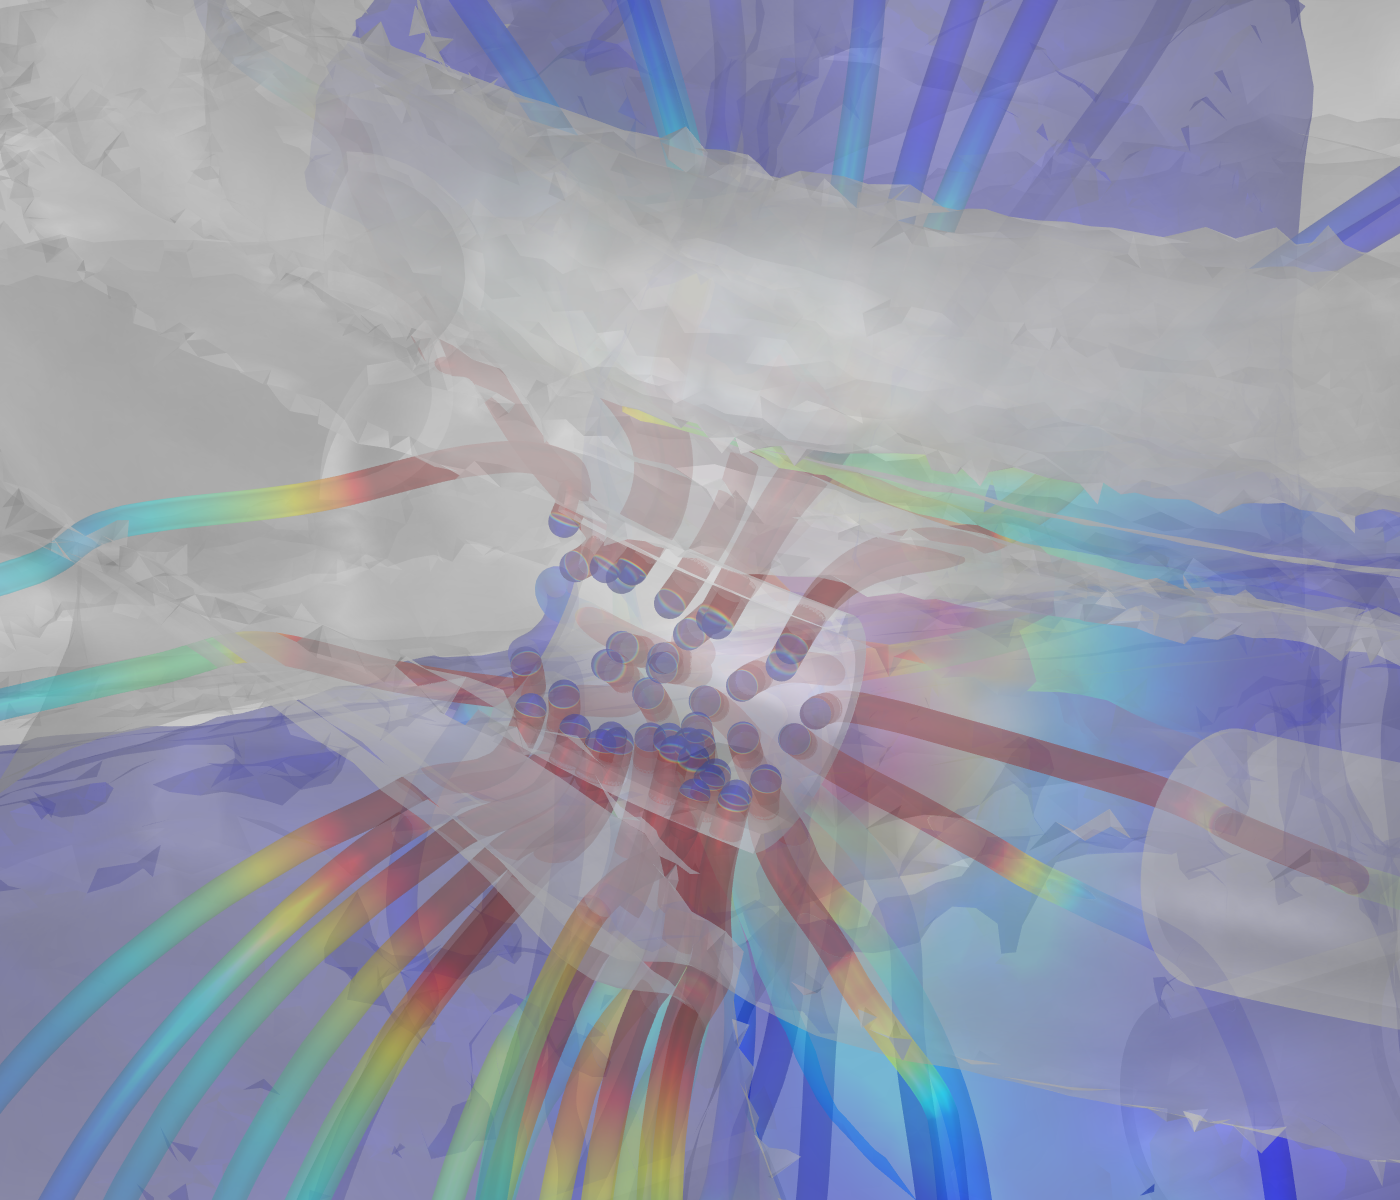
\includegraphics[width=7cm,trim={2cm 2cm 3cm 4cm},clip]
        {Appendix/streamSeedsRand1}
        \caption{On selected boundaries, attempt 1}
        \label{fig:seeding_problem_rand1}
    \end{subfigure}%
	\hfill%
	\begin{subfigure}[t]{0.5\textwidth}
        \centering
        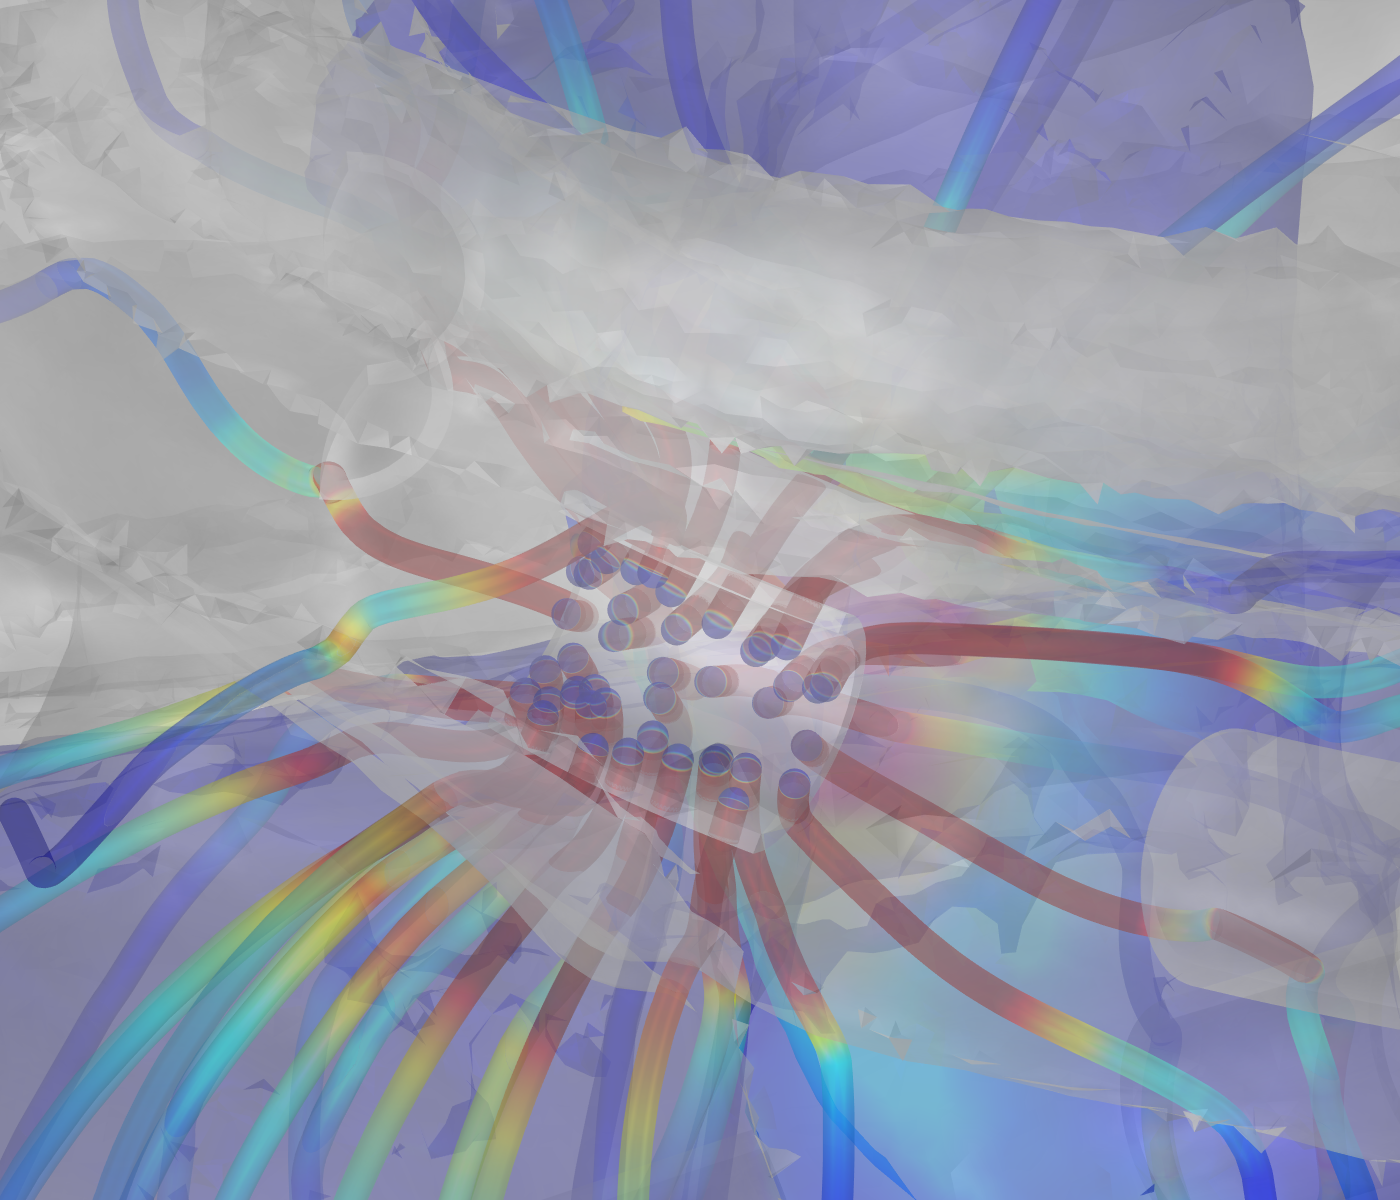
\includegraphics[width=7cm,trim={2cm 2cm 3cm 4cm},clip]
        {Appendix/streamSeedsRand2}
        \caption{On selected boundaries, attempt 2}
        \label{fig:seeding_problem_rand2}
    \end{subfigure}\\%
    \vspace{1em}%
    \begin{subfigure}[t]{0.5\textwidth}
        \centering
        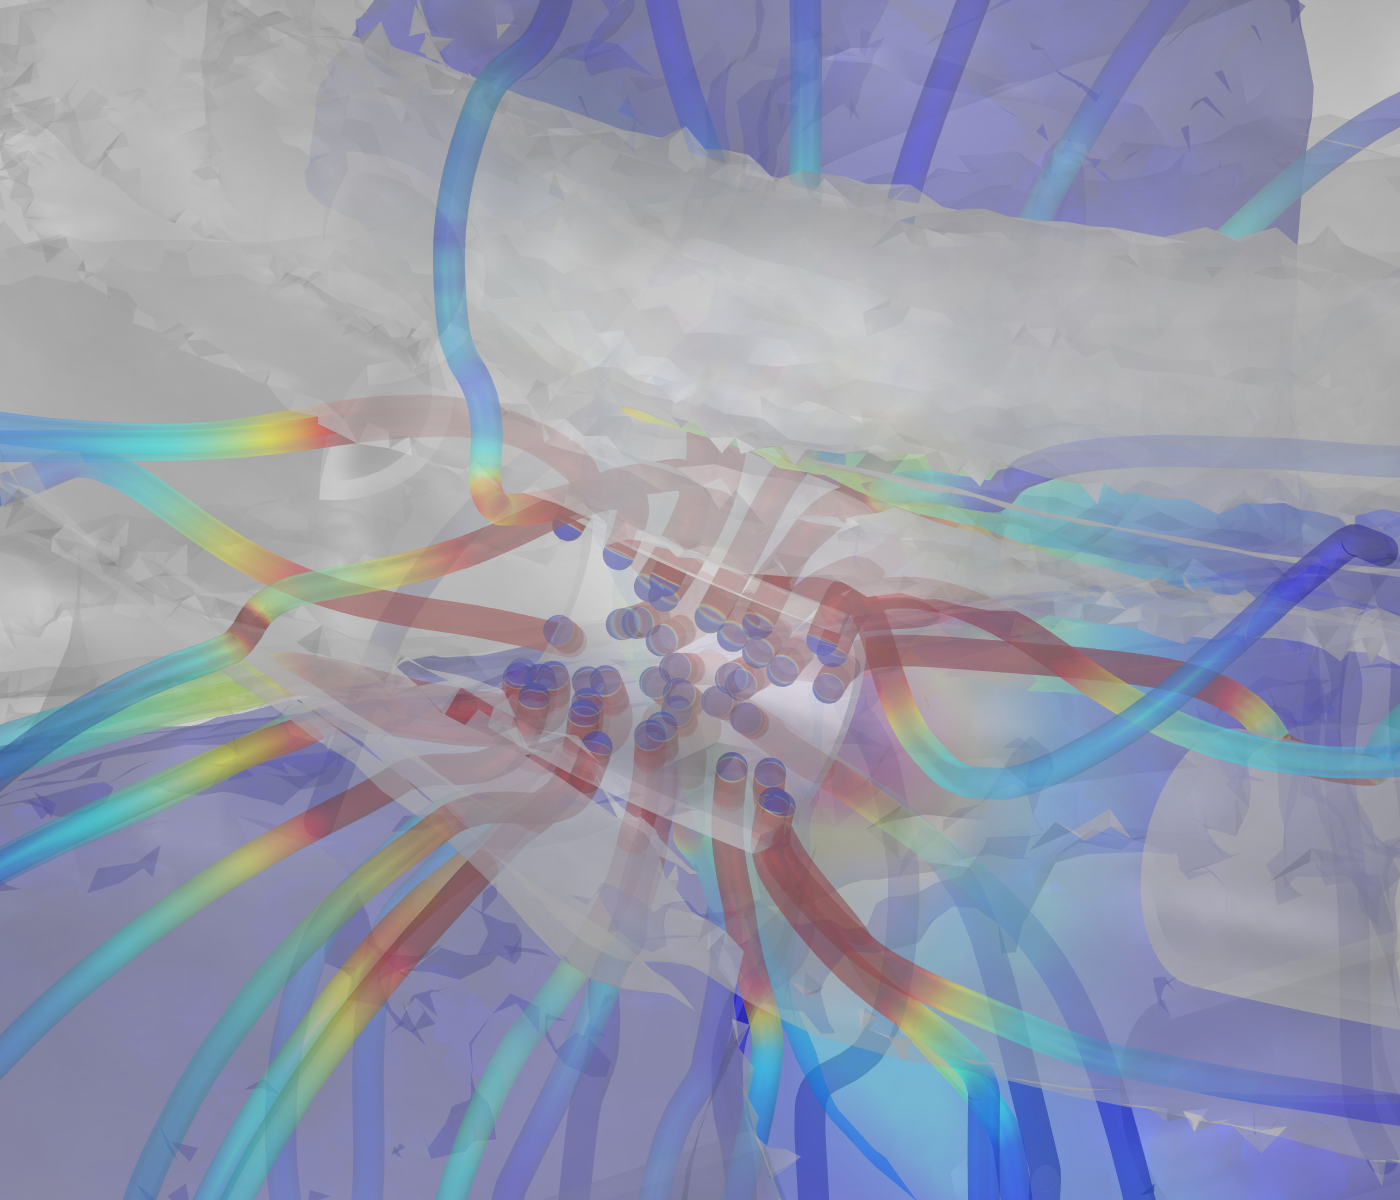
\includegraphics[width=7cm,trim={2cm 2cm 3cm 4cm},clip]
        {Appendix/streamSeedsRand3}
        \caption{On selected boundaries, attempt 3}
        \label{fig:seeding_problem_rand3}
    \end{subfigure}%
    \begin{subfigure}[t]{0.5\textwidth}
        \centering
        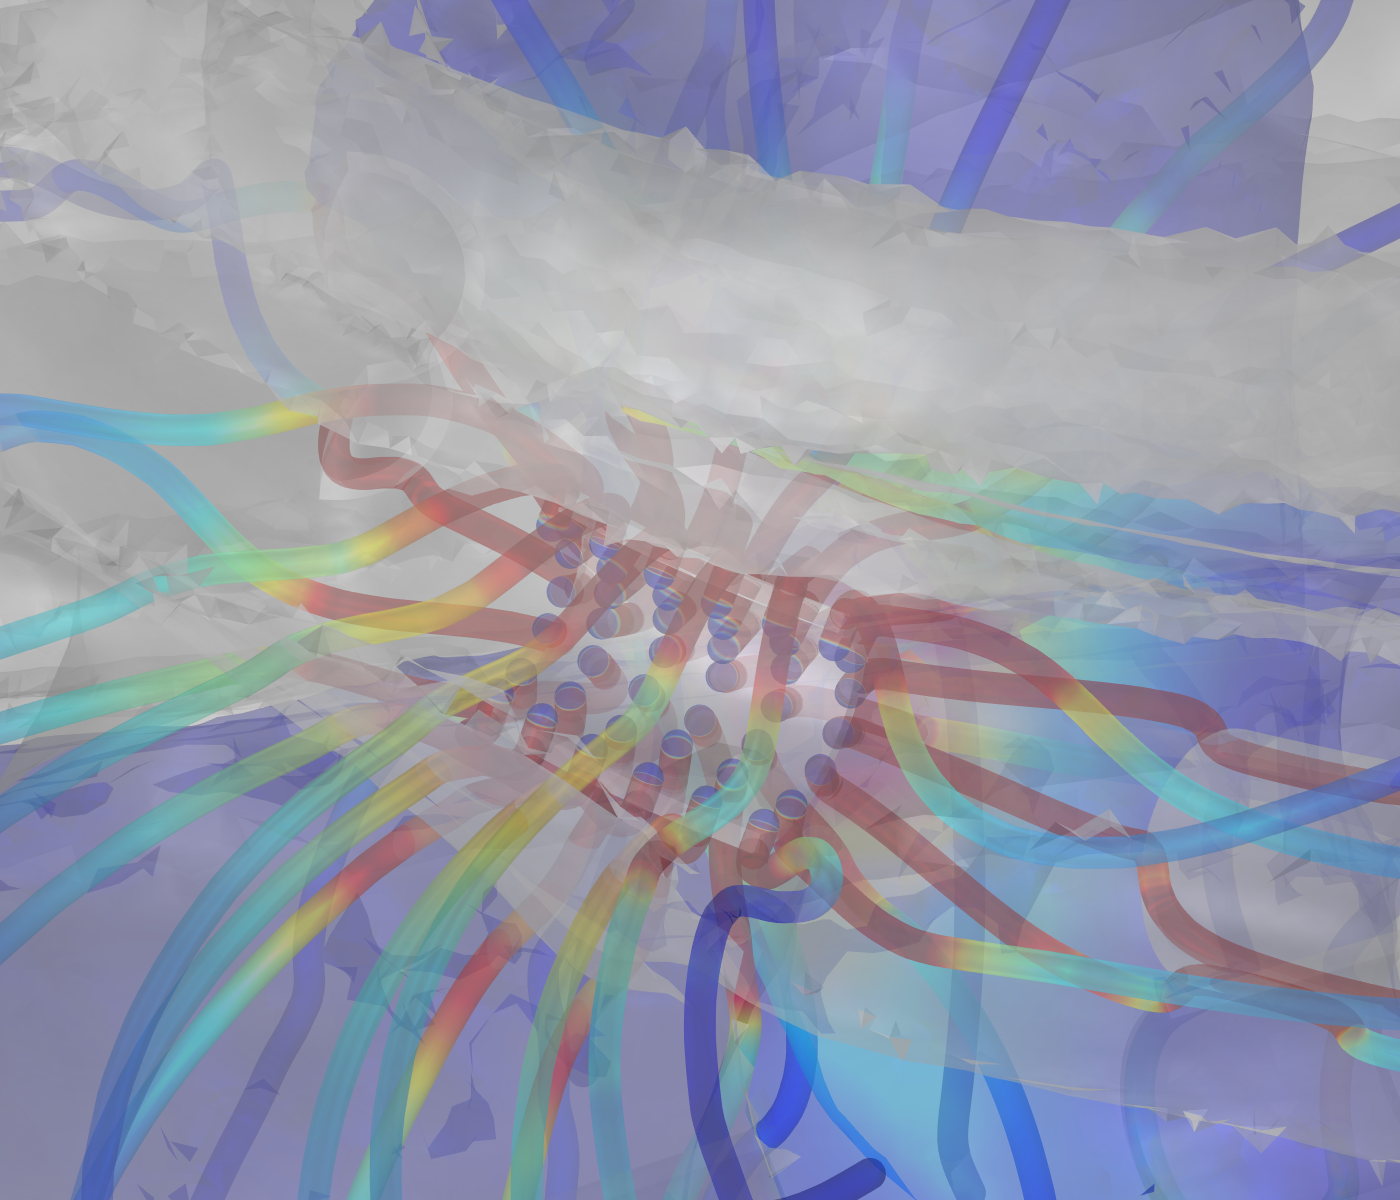
\includegraphics[width=7cm,trim={2cm 2cm 3cm 4cm},clip]
        {Appendix/streamSeedsGrid}
        \caption{Start point controlled}
        \label{fig:seeding_problem_grid}
    \end{subfigure}
    
	\caption[The streamline seeding problem]{The streamline seeding problem. 42
	streamlines are plotted in each case, viewed from the lateral aspect. Note the
	randomised distribution of seed points when plotting on selected boundaries,
	which resulted in a different distribution of streamlines through the volume.}
	\label{fig:seeding_problem}
\end{figure}

% \section{Obtaining Regularly Spaced Seed Points}

In order to provide a more intuitive visualisation, the seed points should
be spaced regularly over the surface of the stimulating electrode. We also
wanted to be able to change the set of seed points programmatically so that the
plots could be customised depending on which electrode was active. In my
discussions with COMSOL Support, they suggested that the only way to achieve
this was to list the coordinates of each seed point manually. As such, a
workaround was developed using the ANSYS suite as follows:

\begin{enumerate}
    \item Import the CAD file for the electrode pads into ICEM CFD.
    \item Perform a ``Build Topology'' operation on the pads to ensure that the
    edges are recognised by the program.
    \item Set the Global Shell Mesh Parameters to generate an ``All Quad'' mesh
    using the ``Autoblock'' method.
    \item Set the element mesh size limits using the Part Mesh Setup box to
    suit the number of streamlines desired. This may require some trial and
    error. Note that it does not have to match the settings used for the
    volume mesh.
    \item Compute the surface mesh. The result should be similar to that
    shown in Figure~\ref{fig:electrode_quad_mesh} (but without the carrier).
    Export the file as a NASTRAN (or STL).
    
    \begin{figure}
	    \centering
	    \begin{subfigure}[t]{0.5\textwidth}
	        \centering
	        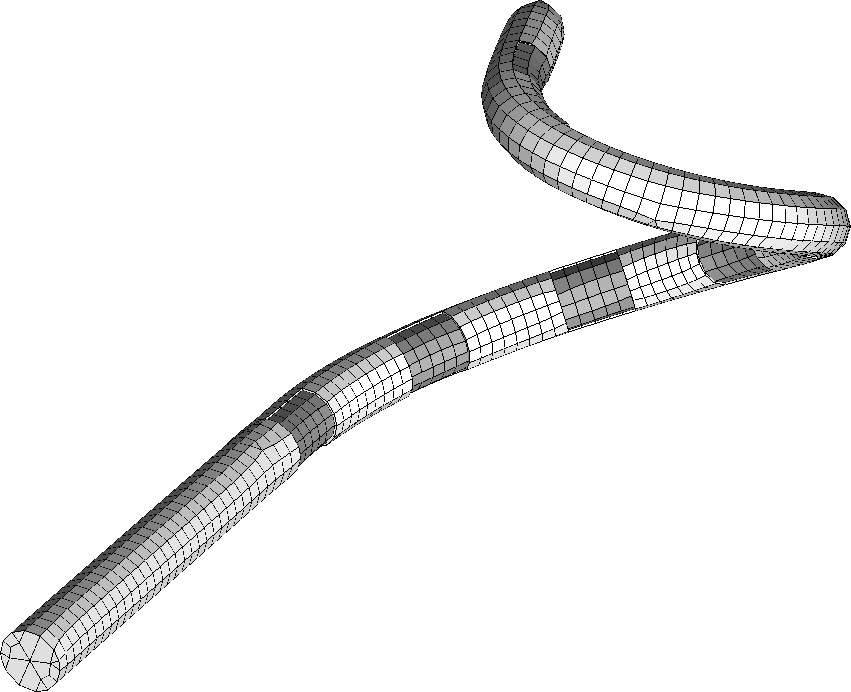
\includegraphics[height=5.5cm]{Appendix/array_autoblock}
	        \caption{Electrode array}
	        \label{fig:array_quad}
	    \end{subfigure}%
		\hfill%
		\begin{subfigure}[t]{0.5\textwidth}
	        \centering
	        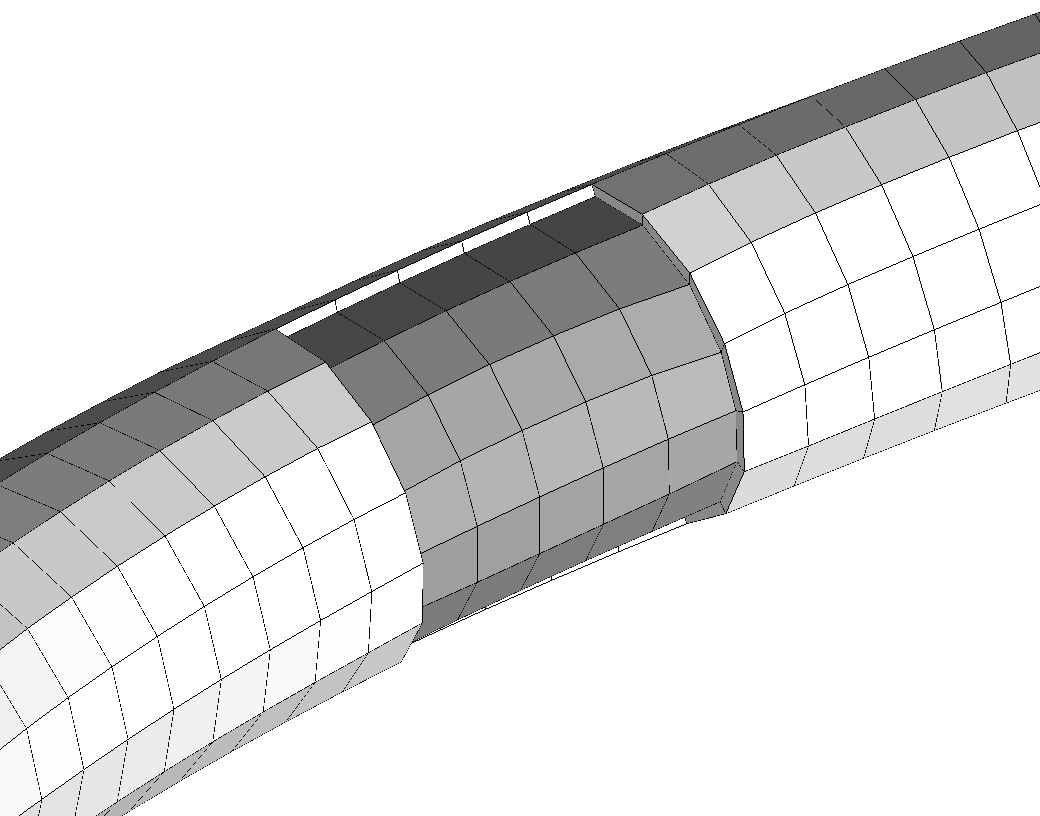
\includegraphics[height=5.5cm]{Appendix/array_autoblock_zoom}
	        \caption{Close up of electrode E2}
	        \label{fig:array_quad_zoom}
	    \end{subfigure}%
	    
		\caption[Quadrilateral mesh of the electrode surface]{Quadrilateral mesh of
		the electrode surface. Here, the silicone carrier is also shown for context.}
		\label{fig:electrode_quad_mesh}
	\end{figure}
    
    \item Open ANSYS Workbench, add an FE Modeller module, and import the
    surface mesh file from ICEM CFD. Perform a visual inspection to check that
    the mesh is correct.
    \item Add a Static Structural module in Workbench and link the surface mesh
    to the model component.
    \item Insert a named selection and select the exposed surface of an
    electrode contact.
    \item Insert a second named selection. Using a worksheet, add the named
    selection from the previous step, then convert to mesh nodes.
    \item Ensure that node locations are included when exporting by checking the
    appropriate option in Workbench. If unsure,
    \href{http://www.eng-tips.com/viewthread.cfm?qid=310295}{see this discussion
    thread}. The relevant comment by Christopher K. Hubley is reproduced
    below.\bigskip
	    \setstretchcode
		\lstinputlisting[]{Code/ansysNodeExport.txt}
		\setstretchnormal
	\item Export the named selection with the nodes as a plain text file. Format
	the data as comma separated (suggest using
	\href{http://www.sublimetext.com/}{Sublime Text} for this) and copy into COMSOL
	as required. Using these coordinates with the ``start point controlled''
	positioning option should result in consistent streamline plots per
	Figure~\ref{fig:seeding_problem_grid}.
	\item Repeat steps 8--11 for the other electrodes.
\end{enumerate}

%% ================================================================== Appendix C

\chapter{Ethics Approval}
\label{appendix:ethics}

The guinea pig voltage tomography experiments conducted by Shefin George under
the supervision of James Fallon at the Bionics Institute in Melbourne, Australia
were approved by the Royal Victorian Eye and Ear Hospital Animal Research and
Ethics Committee (project number 12/250AB, granted 28 February 2012). Shefin was
added to the project as part of an amendment, as per the Final Report attached.

The author was not directly involved with these experiments, but the data were
used for validation of the model as described in Chapter~\ref{sect:validation}.


\includepdf[pages=-]{Appendix/12_250AB-Approval.pdf}

\includepdf[pages=-]{Appendix/12_250AB-FinalReport.pdf}

%% ================================================================== Appendix F

\chapter{Microfil Specification Sheet}
\label{appendix:microfil_specs} % Linked in Vasculature

The official documentation for the Microfil compound used in the microCT imaging
of the vasculature is provided below.

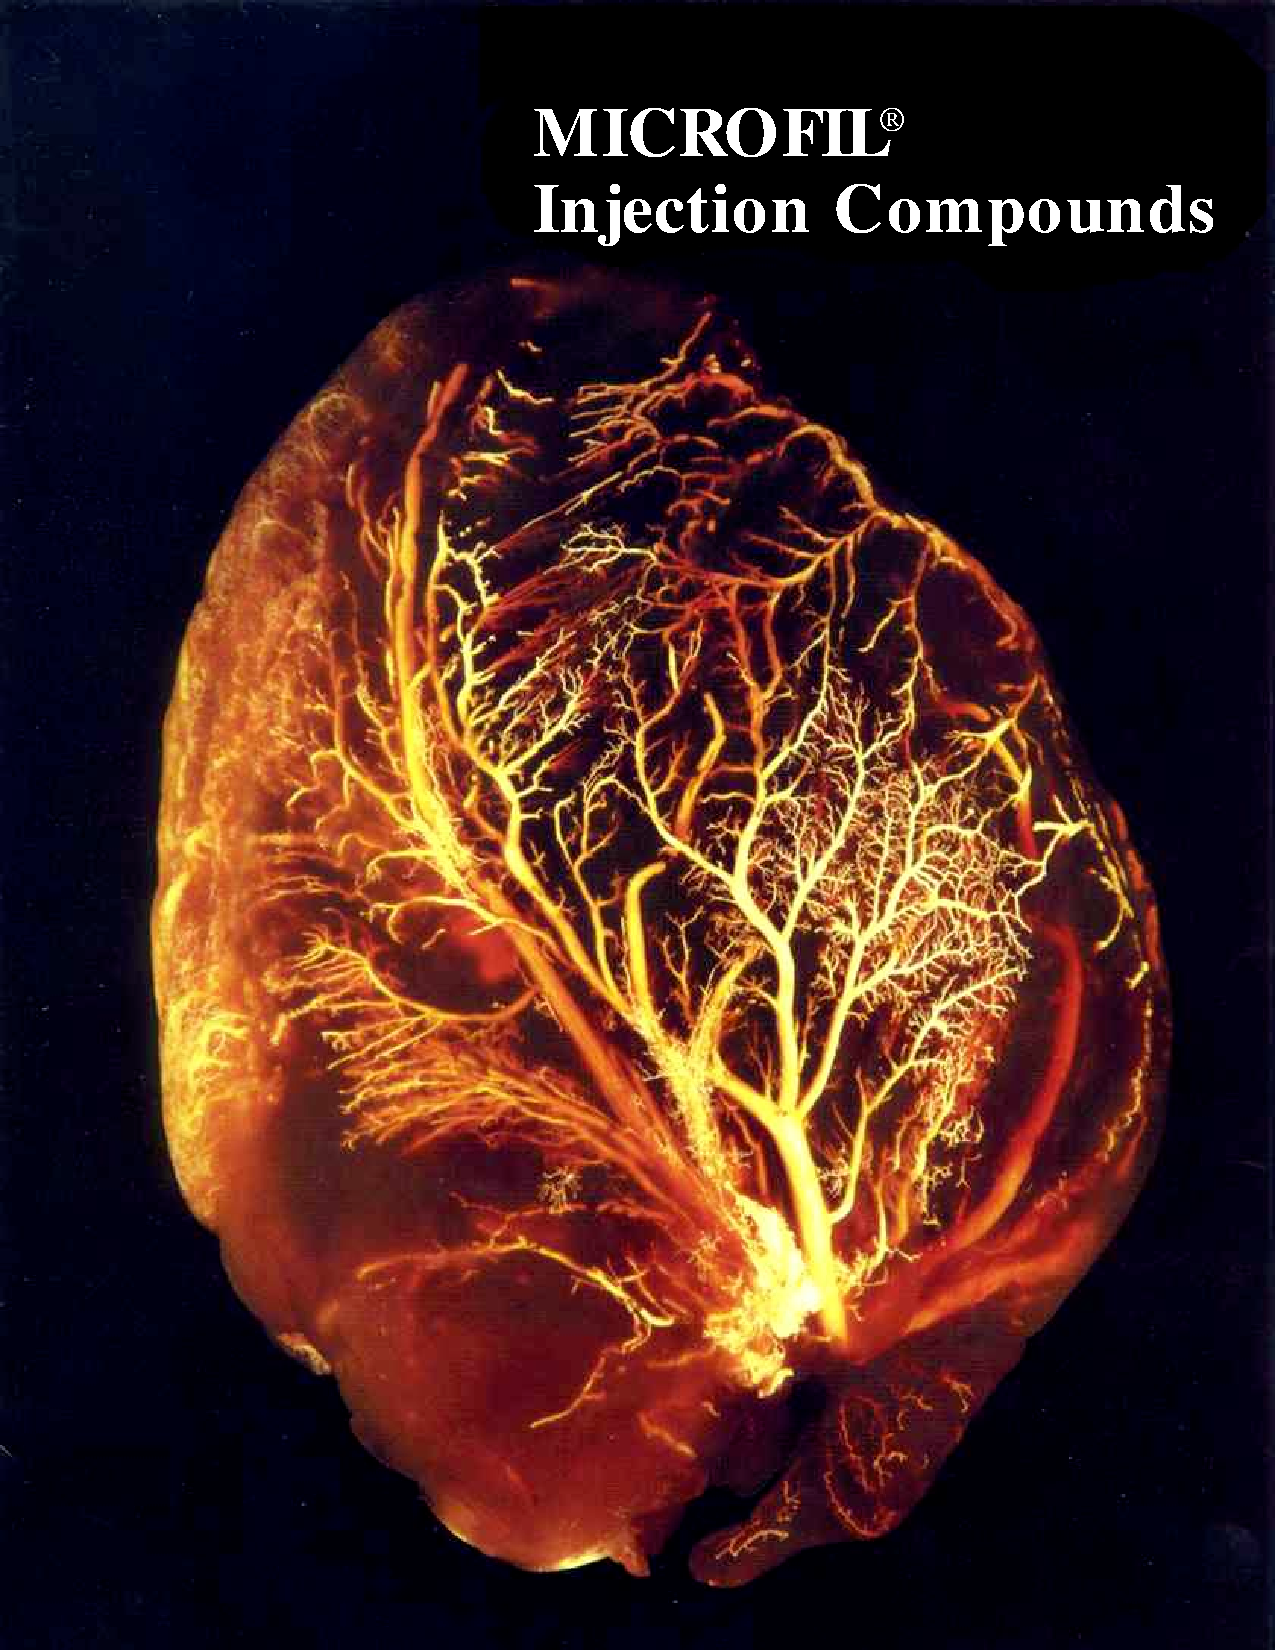
\includepdf[pages=-]{Appendix/MICROFILspecs.pdf}

%% ================================================================== Appendix G

\chapter{Digital Files}
\label{appendix:digital_files} % Linked in Time-dependent Effects

Some additional supplementary files can be accessed online at
\href{http://1drv.ms/1S7qigU}{http://1drv.ms/1S7qigU}.

% Revert formatting
\makeatletter
	\def\toclevel@chapter{0}
\makeatother

\end{appendices}